\section{Fenchel duality and algorithms}

In this section, we introduce the Fenchel conjugate. First, recall that for a real-valued convex function of a single variable $f(x)$, we call $f^*(p) := \sup_x px - f(x)$ its Legendre transform. This is illustrated in figure \ref{fig:leg-conj}.

\begin{figure}[h]
    \centering
    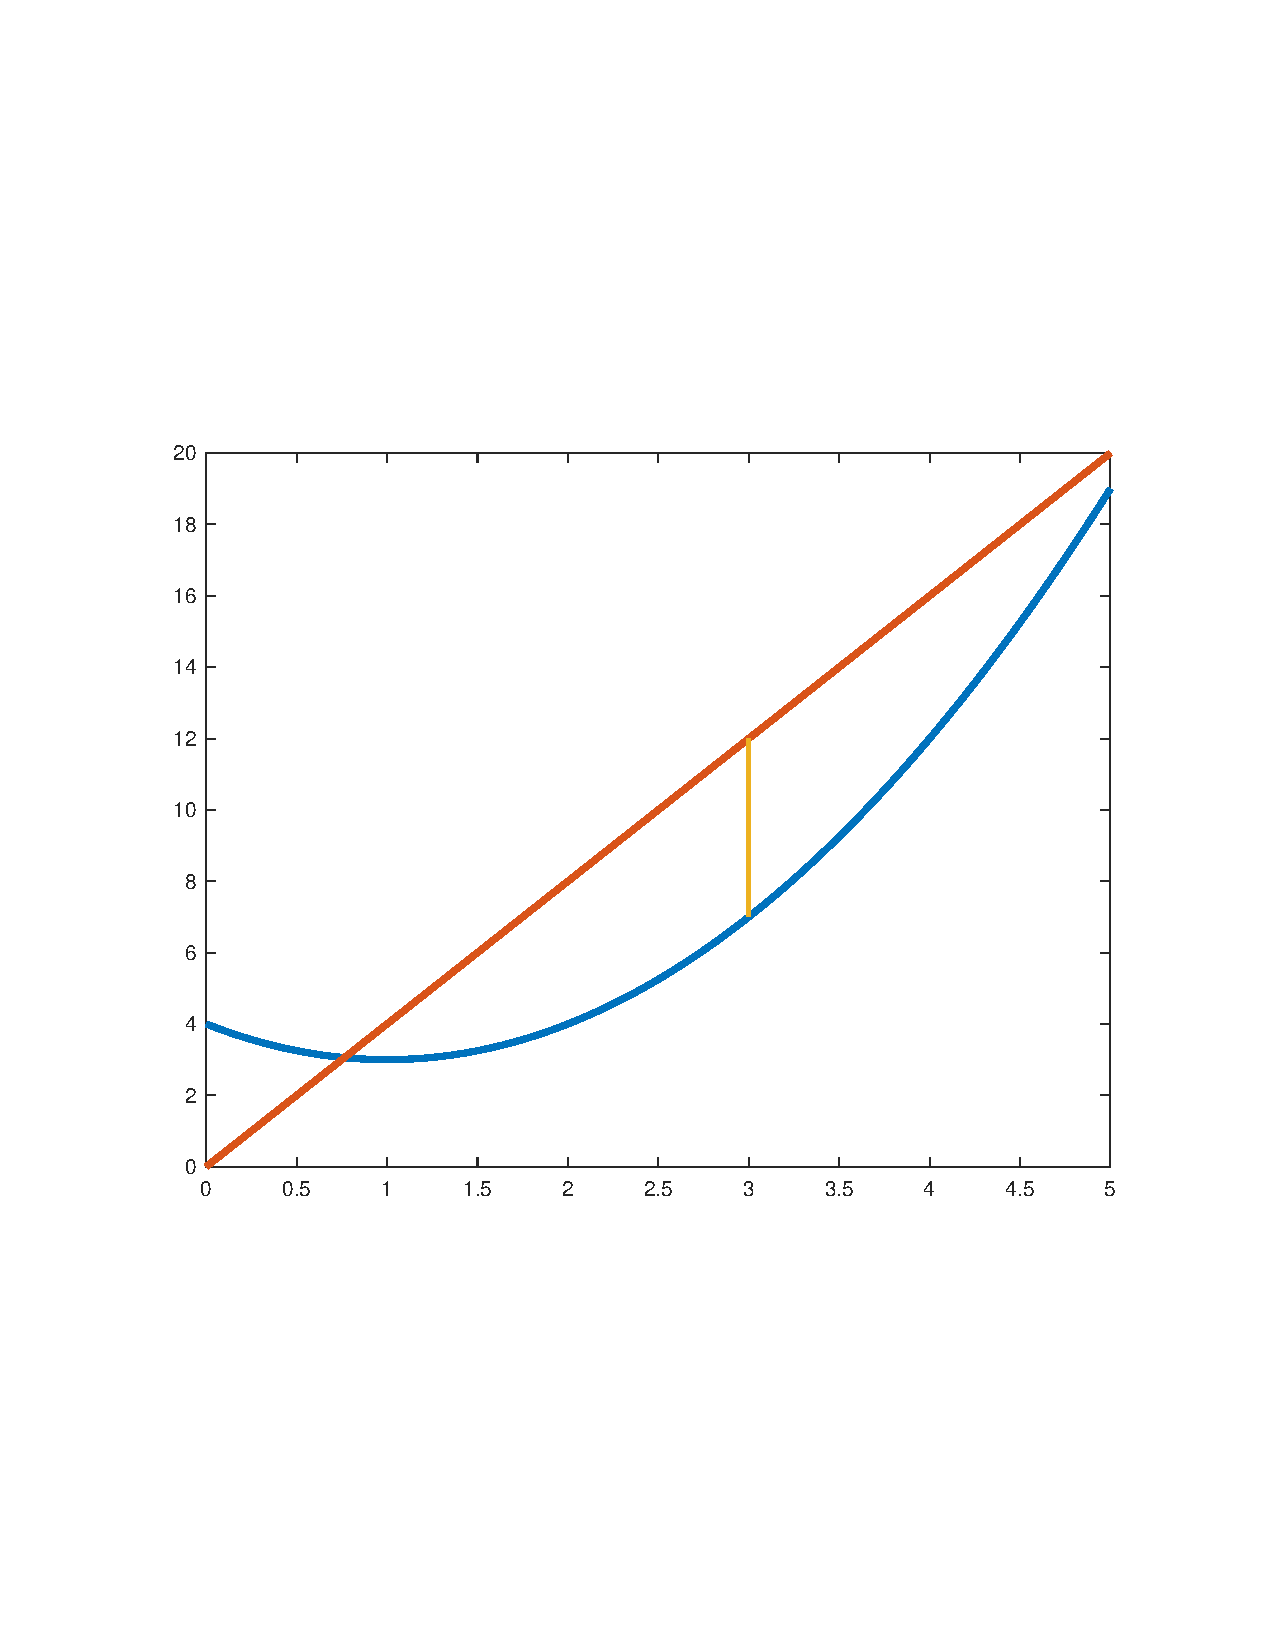
\includegraphics[width=.75\textwidth, trim = 0 200 0 200, clip]{figures/lecture15-conjugate.pdf}
    \caption{Legendre Transform. The function $f^*(p)$ is how much we need to vertically shift the epigraph of $f$ so that the linear function $px$ is tangent to $f$ at $x$.}
    \label{fig:leg-conj}
\end{figure}

The generalization of the Legendre transform to (possibly nonconvex) functions of multiple variables is the Fenchel conjugate.
\begin{definition}[Fenchel conjugate]
The Fenchel conjugate of $f:\R^n \to \R$ is \[f^*(p) = \sup_x \iprod{p,x} - f(x)\]
\end{definition}

We now present several useful facts about the Fenchel conjugate. The proofs are left as an exercise.

\begin{fact}
$f^*$ is convex.
\end{fact}

Indeed, $f^*$ is the supremum of affine functions and therefore convex. Thus, the Fenchel conjugate of $f$ is also known as its convex conjugate.

\begin{fact}
$f^*(f^*(x)) = f$ if $f$ is convex.
\end{fact}

In other words, the Fenchel conjugate is its own inverse for convex functions. Now, we can also relate the subdifferential of a function to that of its Fenchel conjugate. Intuitively, observe that $0 \in \partial f^*(p) \iff 0 \in  p - \partial f(x) \iff p \in \partial f(x)$. This is summarized more generally in the following fact.

\begin{fact}
The subdifferential of $f^*$ at $p$ is $\partial f^*(p) = \{x: p \in \partial f(x)\}$. 
\end{fact}

Indeed, $\partial f^*(0)$ is the set of minimizers of $f$. 

In the following theorem, we introduce Fenchel duality.

\begin{theorem}[Fenchel duality]\label{thm:fenchel}
Suppose we have $f$ proper convex, and $g$ proper concave. Then \[\min_x f(x)- g(x) = \max_p g^*(p) - f^*(p) \]
where $g^*$ is the concave conjugate of $g$, defined as $\inf_x \iprod{p,x} - g(x)$.
\end{theorem}

In the one-dimensional case, we can illustrate Fenchel duality with Figure \ref{fig:fenc_conj}.

	
\begin{figure}[h]
	\centering
		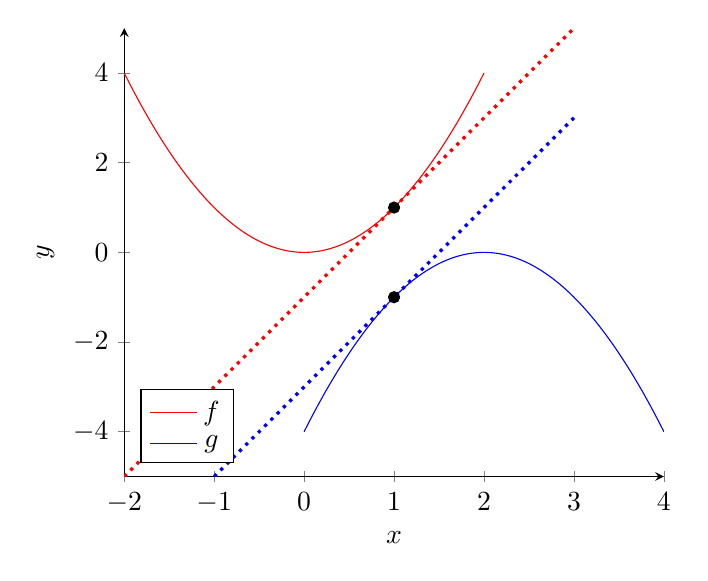
\begin{tikzpicture}
		\begin{axis}[
		axis lines = left,
		xlabel = $x$,
		ylabel = {$y$},
		legend pos=south west,
		]
		%Below the red parabola is defined
		\addplot [
		domain=-2:2, 
		samples=100, 
		color=red,
		]
		{x^2};
		\addlegendentry{$f$}
		%Here the blue parabola is defined
		\addplot [
		domain=0:4, 
		samples=100, 
		color=blue,
		]
		{-1*(x-2)^2};
		\addlegendentry{$g$}
		
		\addplot [
		domain=-1:3, 
		samples=100, 
		color=blue,
		dotted,very thick
		]
		{2*x-3};
		
		\addplot [
		domain=-2:3, 
		samples=100, 
		color=red,
		dotted, very thick
		]
		{2*x-1};
		
		\filldraw[black]  (axis cs:1,1) circle (2pt) ;
		\filldraw[black]  (axis cs:1,-1) circle (2pt);
		
		\end{axis}
		\end{tikzpicture}
		\caption{Fenchel duality in one dimension}\label{fig:fenc_conj}
\end{figure}

In the minimization problem, we want to find $x$ such that the vertical distance between $f$ and $g$ at $x$ is as small as possible. In the (dual) maximization problem, we draw tangents to the graphs of $f$ and $g$ such that the tangent lines have the same slope $p$, and we want to find $p$ such that the vertical distance between the tangent lines is as large as possible. The duality theorem above states that strong duality holds, that is, the two problems have the same solution.

We can recover Fenchel duality from Lagrangian duality, which we have already studied. To do so, we need to introduce a constraint to our minimization problem in Theorem \ref{thm:fenchel}. A natural reformulation of the problem with a constraint is as follows.
\begin{equation}
    \min_{x,z} f(x)-g(z) \text{ subject to } x=z
\end{equation}



\subsection{Deriving the dual problem for empirical risk minimization}
In empirical risk minimization, we often want to minimize a function of the following form:
\begin{equation}
    P(w) = \sum_{i=1}^m \phi_i(\iprod{w,x_i}) + R(w)
\end{equation}

We can think of $w \in \R^n$ as the model parameter that we want to optimize over (in this case it corresponds to picking a hyperplane), and $x_i$ as the features of the $i$-th example in the training set. $\phi_i(\cdot, x_i)$ is the loss function for the $i$-th training example and may depend on its label. $R(w)$ is the regularizer, and we typically choose it to be of the form $R(w) = \frac{\lambda}{2}\norm{w}^2$.

The primal problem, $\min_{w\in \R^n}P(w)$, can be equivalently written as follows:
\begin{equation}
    \min_{w,z}  \sum_{i=1}^m \phi_i(z_i) + R(w) \text{ subject to } X^\top w=z
\end{equation}
By Lagrangian duality, we know that the dual problem is the following:
\begin{align*}
    &\max_{\alpha \in \R^m} \min_{z,w} \sum_{i=1}^m \phi_i(z_i) + R(w) - \alpha^\top(X^\top w-z) \\
    =&\max_\alpha \min_{w,z} \sum_{i=1}^m \phi_i(z_i) + \alpha_iz_i + R(w) - \alpha^\top X^\top w \\
    =&\max_\alpha \left(- \min_{w,z} - \left(\sum_{i=1}^m \phi_i(z_i)  + \alpha_iz_i \right) + (X\alpha)^\top w -R(w) \right) \\
    =& \max_\alpha - \left( \sum_{i=1}^m \max_{z_i} \left( - \phi_i(z_i) - \alpha_iz_i \right) + \max_w (X\alpha)^\top w - R(w)    \right) \\
    =& \max_\alpha -\sum_{i=1}^n \phi_i^*(-\alpha_i) -R^*(X\alpha)
\end{align*}
where $\phi_i^*$ and $R^*$ are the Fenchel conjugates of $\phi_i$ and $R^*$ respectively.
Let us denote the dual objective as $D(\alpha) = \sum_{i=1}^m \phi_i^*(-\alpha_i) - R^*(X\alpha)$. By weak duality, $D(\alpha) \leq P(w)$.

For $R(w) = \frac{\lambda}{2}\norm{w}^2$, $R^*(p) = \frac{\lambda}{2} \norm{\frac{1}{\lambda} p}^2$. So $R$ is its own convex conjugate (up to correction by a constant factor). In this case the dual becomes:
\[\max_\alpha \sum_{i=1}^m \phi_i^*(-\alpha_i) - \frac{\lambda}{2} \norm{\frac{1}{\lambda} \sum_{i=1}^m \alpha_ix_i}^2 \]

We can relate the primal and dual variables by the map $w(\alpha) = \frac{1}{\lambda} \sum_{i=1}^m \alpha_ix_i$. In particular, this shows that the optimal hyperplane is in the span of the data. Here are some examples of models we can use under this framework.

\begin{example}[Linear SVM]
We would use the hinge loss for $\phi_i$. This corresponds to \[\phi_i(w) = \max(0,1-y_ix_i^\top w)~,\quad -\phi_i^*(-\alpha_i) = \alpha_i y_i\]
\end{example}

\begin{example}[Least-squares linear regression]
We would use the squared loss for $\phi_i$. This corresponds to \[\phi_i(w) = (w^\top x_i-y_i)^2~,\quad -\phi_i^*(-\alpha_i) = \alpha_i y_i + \alpha^2/4\]
\end{example}

We end with a fact that relates the smoothness of $\phi_i$ to the strong convexity of $\phi_i^*$.

\begin{fact}
If $\phi_i$ is $\frac{1}{\gamma}$-smooth, then $\phi^*_i$ is $\gamma$-strongly convex.
\end{fact}

\subsection{Stochastic dual coordinate ascent (SDCA)}

In this section we discuss a particular algorithm for empirical risk minimization which makes use of Fenchel duality. Its main idea is picking an index $i\in[m]$ at random, and then solving the dual problem at coordinate $i$, while keeping the other coordinates fixed.

More precisely, the algorithm performs the following steps:
\begin{enumerate}
\item Start from $w^0:=w(\alpha^0)$
\item For $t=1,\dots, T$:
    \begin{enumerate}
        \item Randomly pick $i\in[m]$
        \item Find $\Delta\alpha_i$ which maximizes
        $$-\Phi_i\left(-(\alpha_i^{t-1}+\Delta\alpha_i)\right)-\frac{\lambda}{2m}\Norm{w^{t-1}+\frac{1}{\lambda}\Delta\alpha_ix_i}^2$$
    \end{enumerate}
\item Update the dual and primal solution
    \begin{enumerate}
        \item $\alpha^t = \alpha^{t-1}+\Delta\alpha_i$
        \item $w^t = w^{t-1} + \frac{1}{\lambda} \Delta\alpha_ix_i$
    \end{enumerate}
\end{enumerate}
For certain loss functions, the maximizer $\Delta\alpha_i$ is given in closed form. For example, for hinge loss it is given explicitly by:
$$\Delta\alpha_i = y_i\max\left(0,\min(1,\frac{1-x_i^Tw^{t-1}y_i}{\|x_i\|^2/\lambda m} + \alpha_i^{t-1}y_i)\right) - \alpha_i^{t-1},$$
and for squared loss it is given by:
$$\Delta\alpha_i = \frac{y_i - x_i^Tw^{t-1} - 0.5\alpha_i^{t-1}}{0.5 + \|x\|^2/\lambda m}.$$
Note that these updates require both the primal and dual solutions to perform the update.

Now we state a lemma given in $\cite{shalev2013}$, which implies linear convergence of SDCA. In what follows, assume that $\|x_i\|\leq 1$, $\Phi_i(x)\geq 0$ for all $x$, and $\Phi_i(0)\leq 1$.

\begin{lemma}
\lemmalabel{sdcaconv}
Assume $\Phi_i^*$ is $\gamma$-strongly convex, where $\gamma>0$. Then:
$$\Esymb[D(\alpha^t)-D(\alpha^{t-1})]\geq\frac{s}{m}\Esymb[P(w^{t-1})-D(\alpha^{t-1})],$$
where $s=\frac{\lambda m\gamma}{1 + \lambda m \gamma}$.
\end{lemma}
We leave out the proof of this result, however give a short argument that proves linear convergence of SDCA using this lemma. Denote $\epsilon_D^t:=D(\alpha^*) - D(\alpha^t)$. Because the dual solution provides a lower bound on the primal solution, it follows that:
$$\epsilon_D^t \leq P(w^t) - D(\alpha^t).$$
Further, we can write:
$$D(\alpha^t)-D(\alpha^{t-1}) = \epsilon_D^{t-1}-\epsilon_D^t.$$
By taking expectations on both sides of this equality and applying \lemmaref{sdcaconv}, we obtain:
\begin{align*}
\Esymb[\epsilon_D^{t-1}-\epsilon_D^t]&=\Esymb[D(\alpha^t)-D(\alpha^{t-1})]\\
&\geq\frac{s}{m}\Esymb[P(w^{t-1}) - D(\alpha^{t-1})]\\
&\geq\frac{s}{m}\Esymb[\epsilon_D^{t-1}].
\end{align*}
Rearranging terms and recursively applying the previous argument yields:
$$\Esymb[\epsilon_D^t]\leq (1-\frac{s}{m})\Esymb[\epsilon_D^{t-1}]\leq (1-\frac{s}{m})^t\epsilon_D^0.$$
From this inequality we can conclude that we need $O(m+\frac{1}{\lambda\gamma}\log(1/\epsilon))$ steps to achieve $\epsilon$ dual error.

Using \lemmaref{sdcaconv}, we can also bound the primal error. Again using the fact that the dual solution underestimates the primal solution, we provide the bound in the following way:
\begin{align*}
    \Esymb[P(w^t)-P(w^*)]&\leq \Esymb[P(w^t)-D(\alpha^t)]\\
    &\leq\frac{m}{s}\Esymb[D(\alpha^{t+1})-D(\alpha^t)]\\
    &\leq\frac{m}{s}\Esymb[\epsilon_D^t],
\end{align*}
where the last inequality ignores the negative term $-\Esymb[\epsilon_D^{t-1}].$
